%! TeX program = lualatex
\documentclass[third]{../altarcard}

\usepackage[paperheight=12in,paperwidth=18in,margin=0in]{geometry}

%%%%%%%%%%%%%%%%%%%%%%%%%%%%%%%%%%%%%%%%%%%%%%%%%%%%%%%%%%%%%%%%%%%%%%%%%%%%%%%%

\begin{document}

\begin{center}

	\begin{minipage}[t]{0.29\linewidth}

		\vspace*{2.2cm}

		\initial{\hspace*{2cm}G}{loria} in~excelsis \bend{Deo}. Et~in~terra pax
		hominibus bonae voluntatis. Laudamus te. Benedicimus te. \bend{Adoramus
			te}. Glorificamus te. \bend{Gratias agimus tibi} propter magnam gloriam
		tuam. Domine Deus, Rex caelestis, Deus Pater omnipotens. Domine Fili
		unigenite, \bend{Jesu Christe}. Domine Deus, Agnus Dei, Filius Patris.
		Qui tollis peccata mundi, miserere nobis. Qui tollis peccata mundi,
		\bend{suscipe deprecationem nostram}. Qui sedes ad~dexteram Patris,
		miserere nobis. Quoniam tu solus Sanctus. Tu solus Dominus. Tu solus
		Altissimus, \bend{Jesu Christe}. Cum Sancto \cross~ Spiritu in~gloria
		Dei Patris. \amen

		\gap

		\initial{M}{unda} cor meum, ac~labia mea, omnipotens Deus, qui labia
		Isaiae Prophetae calculo mundasti ignito: ita me~tua grata miseratione
		dignare mundare, ut~sanctum Evangelium tuum digne valeam nuntiare. Per
		Christum Dominum nostrum. \amen

		\gap

		\initial{I}{ube}, Domine benedicere. Dominus sit in~corde meo et~in~
		labiis meis: ut~digne et~competenter annuntiem Evangelium suum. \amen

		\gap

		\initial{C}{redo} in~unum \bend{Deum}, Patrem omnipotentem, factorem
		caeli et~terrae, visibilium omnium, et~invisibilium. Et~in~unum Dominum
		\bend{Jesum Christum}, Filium Dei unigenitum. Et~ex Patre natum ante
		omnia saecula. Deum de~Deo, lumen de~lumine, Deum verum de~Deo vero.
		Genitum, non factum, consubstantialem Patri: per quem omnia facta sunt.
		Qui propter nos homines, et~propter nostram salutem descendit de~caelis.
		\textcolor{Maroon}{\bfseries\scshape Et~incarnatus est de~spiritu sancto
			ex~maria virgine: et~homo factus est.} Crucifixus etiam pro nobis, sub
		Pontio Pilato passus, et~sepultus est. Et~resurrexit tertia die,
		secundum Scripturas. Et~ascendit in~caelum: sedet ad~dexteram Patris.
		Et~iterum venturus est cum gloria, judicare vivos, et~mortuos: cujus
		regni non erit finis. Et~in~Spiritum Sanctum, Dominum et~vivificantem:
		qui ex~Patre Filioque procedit. Qui cum Patre et~Filio \bend{simul
			adoratur} et~conglorificatur: qui locutus est per Prophetas. Et~unam,
		sanctam, catholicam et~apostolicam Ecclesiam. Confiteor unum baptisma
		in~remissionem
		% 
		\hspace*{2cm} \parbox{0.85\linewidth}{ \smallskip peccatorum.
			Et~exspecto resurrectionem mortuorum. Et~vitam \cross~venturi saeculi.
			\amen}

		% \vspace*{0.25em}
		% \hfill
		% \begin{minipage}{0.85\linewidth}
		% 	peccatorum. Et~exspecto resurrectionem mortuorum. Et~vitam \cross~venturi
		% 	saeculi.
		% 	\amen
		% \end{minipage}


	\end{minipage}
	\hspace*{0.8cm}
	\begin{minipage}[t]{0.25\linewidth}
		%
		\vspace*{2.2cm}
		%
		\begin{center}
			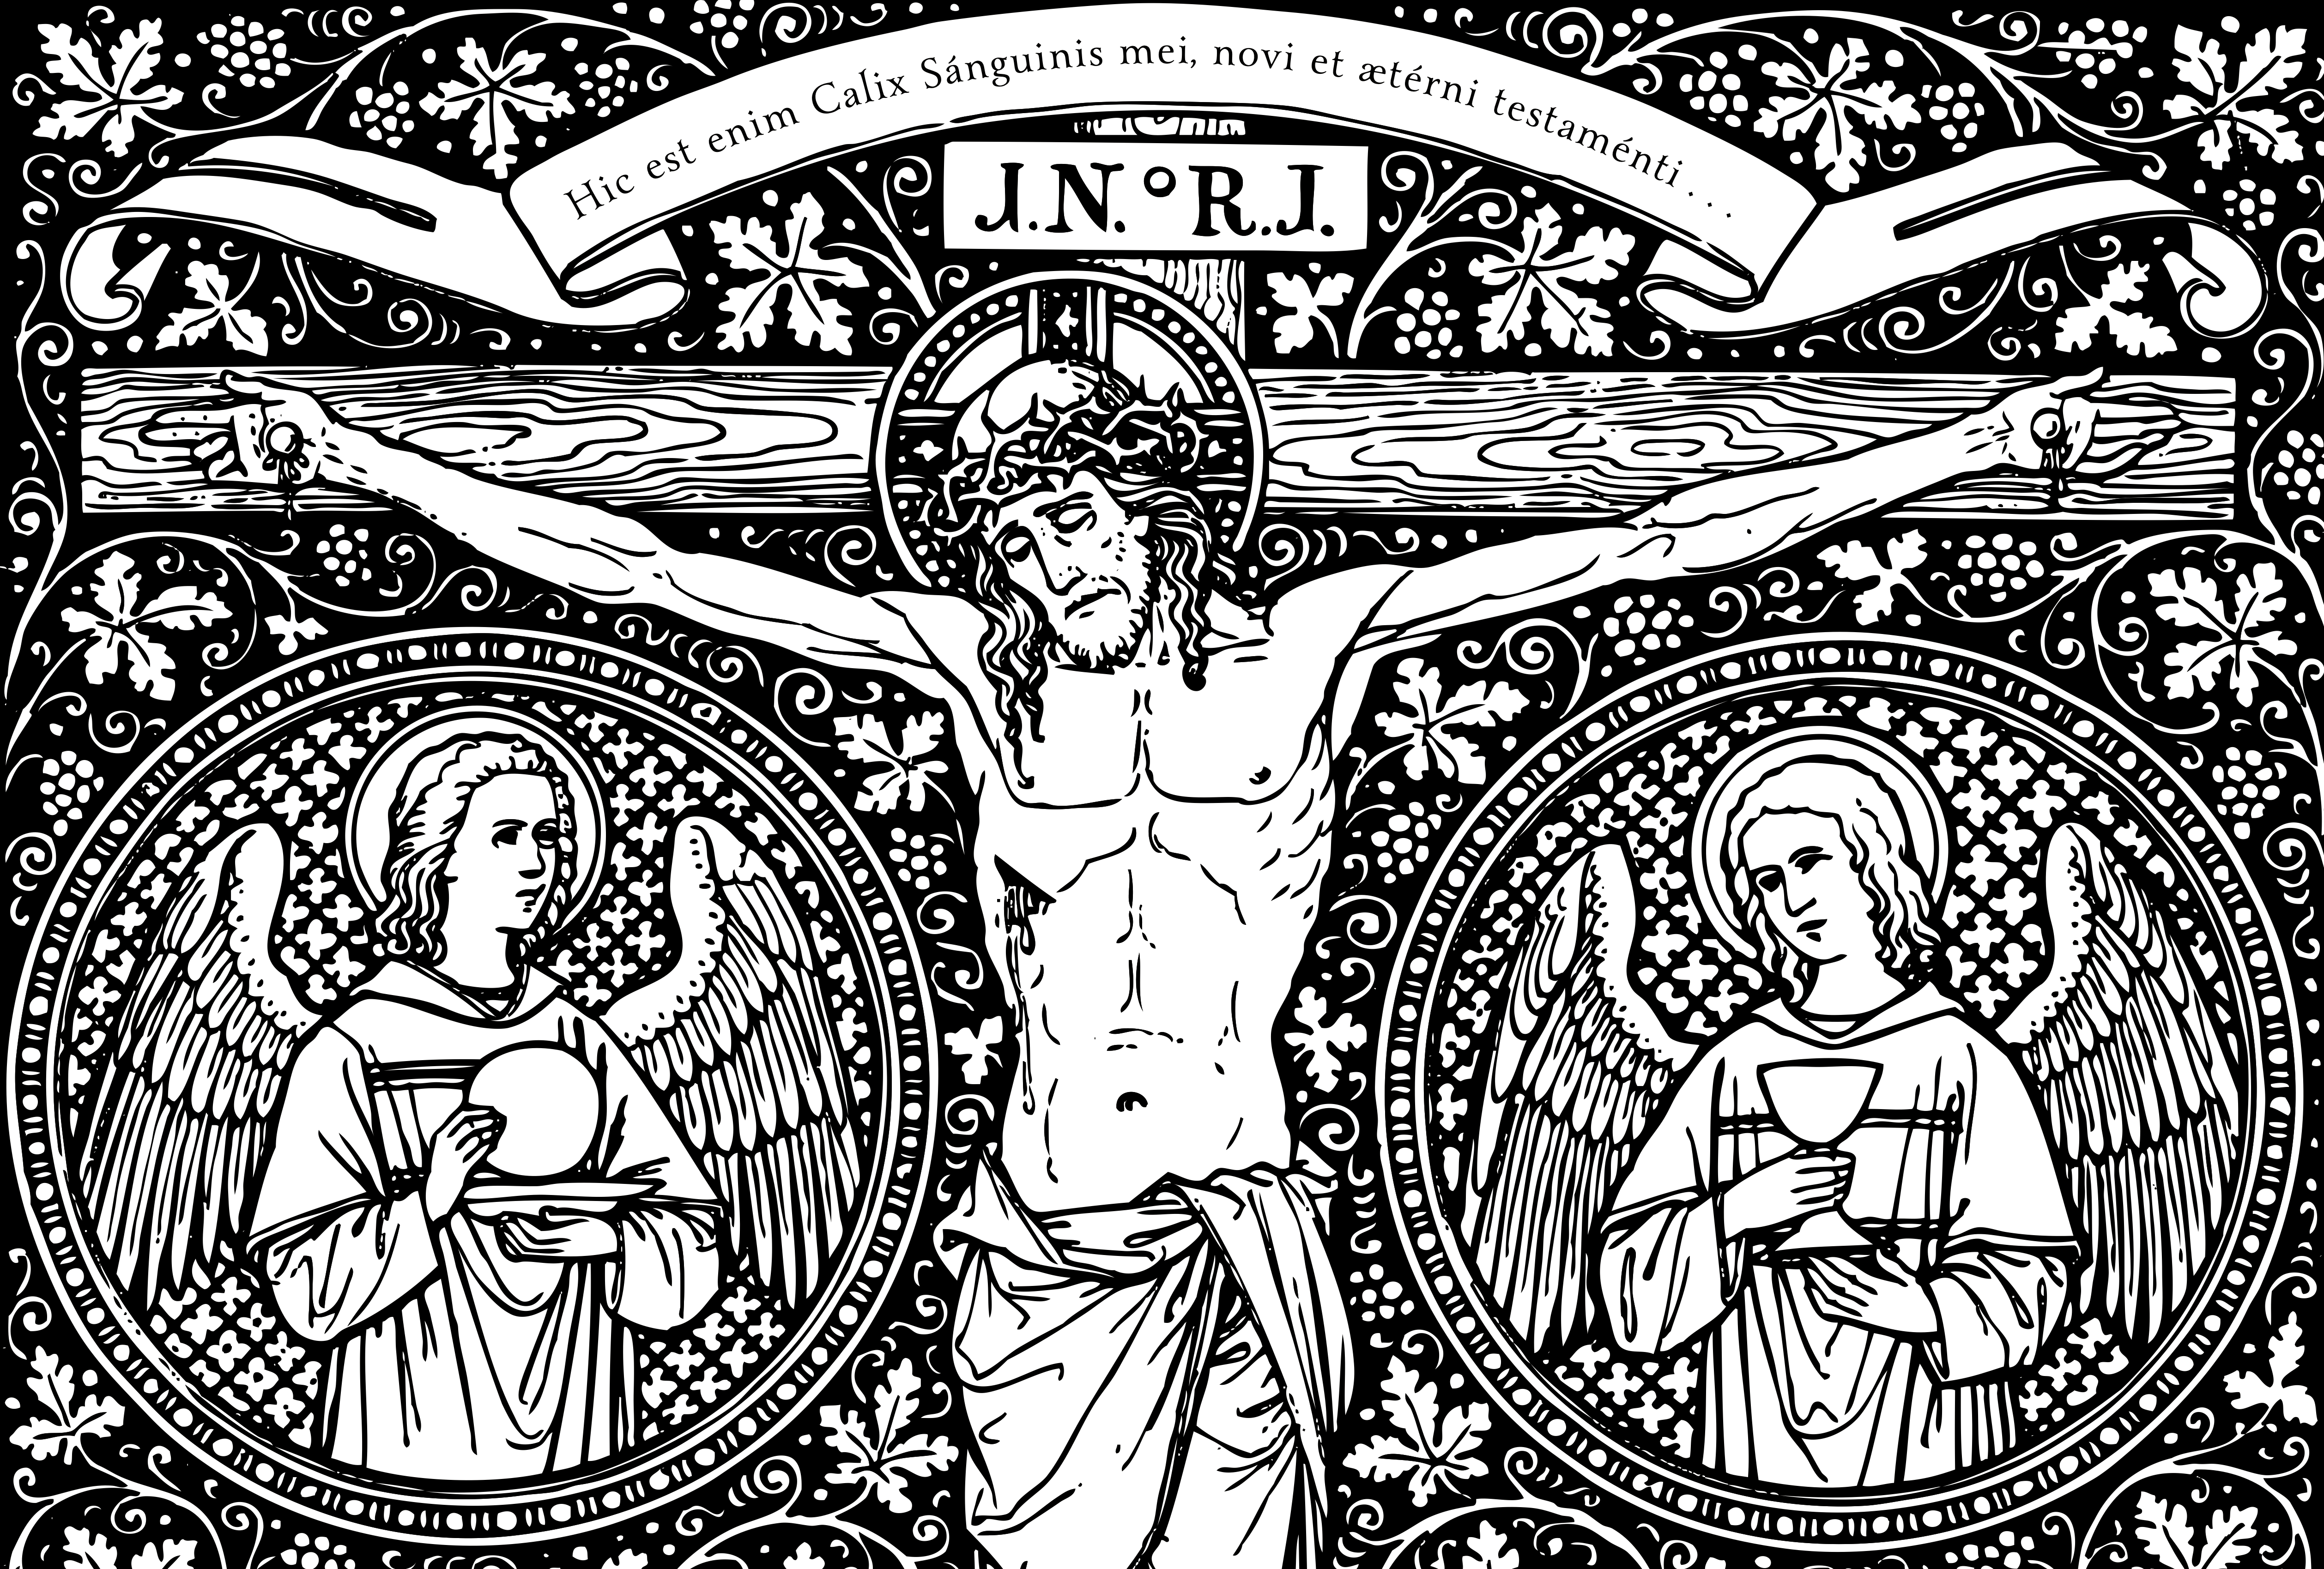
\includegraphics[width=\linewidth]{../Figures/krzyz.png}
		\end{center}
		%
		\bigskip
		%
		\lettrine[lines=3,depth=1]{\color{Maroon}Q}{\bfseries\color{Maroon}ui}
		pridie quam pateretur, accepit panem in~sanctas ac~venerabiles manus
		suas, et~elevatis oculis in~caelum ad~te Deum Patrem suum omnipotentem,
		tibi gratias agens, bene\cross dixit, fregit, deditque discipulis sui
		dicens: Accipite, et~manducate ex~hoc omnes:\\

		\medskip

		\centerline{\begin{minipage}{0.75\linewidth}
				\begin{center}
					\Large\color{Maroon}\bfseries\scshape
					%
					Hoc est enim Corpus meum.
				\end{center}
			\end{minipage}}

		\medskip

		\initial{S}{imili} modo postquam coenatum est, accipiens et~hunc
		praeclarum Calicem in~sanctas ac~venerabiles manus suas: item tibi
		gratias agens, bene\cross dixit, deditque discipulis suis, dicens:
		Accipite, et~bibite ex~eo omnes:\\

		\medskip

		\centerline{\begin{minipage}{0.75\linewidth}
				\begin{center}
					\Large\color{Maroon}\bfseries\scshape
					%
					Hic est enim Calix Sanguinis mei, novi et~aeterni
					testamenti: mysterium fidei: qui pro vobis et~pro multis
					effundetur in~remissionem peccatorum.
				\end{center}
			\end{minipage}}

		\medskip

		\centerline{\begin{minipage}{\linewidth}
				Haec quotiescumque feceritis, in~mei memoriam facietis.
			\end{minipage}}

	\end{minipage}
	\hspace*{0.8cm}
	\begin{minipage}[t]{0.29\linewidth}

		\vspace*{2.2cm}

		% \begin{minipage}{0.85\linewidth}
		% 	\initial{S}{uscipe}, sancte Pater, omnipotens aeterne Deus, hanc
		% 	immaculatam hostiam, quam ego indignus famulus tuus offero tibi Deo meo
		% 	vivo et~vero,
		% \end{minipage}
		% \vspace*{0.25em}

		\parbox{0.87\linewidth}{\initial{S}{uscipe}, sancte Pater, omnipotens
			aeterne Deus, hanc immaculatam hostiam, quam ego indignus famulus
			tuus offero tibi Deo meo vivo et~vero, pro}

		\smallskip

		innumerabilibus peccatis, et~offensionibus, et~negligentiis meis,
		et~pro omnibus circumstantibus, sed et~pro omnibus fidelibus Christianis
		vivis atque defunctis: ut~mihi, et~illis proficiat ad~salutem in~vitam
		aeternam.
		\amen

		\gap

		\initial{O}{fferimus} tibi, Domine, calicem salutaris, tuam deprecantes
		clementiam: ut~in~conspectu divinae majestatis tuae, pro nostra, et
		totius mundi salute cum odore suavitatis ascendat. \amen

		\gap

		\initial{I}{n} spiritu humilitatis, et~in~animo contrito suscipiamur a
		te, Domine: et~sic fiat sacrificium nostrum in~conspectu tuo hodie, ut
		placeat tibi, Domine Deus

		\gap

		\initial{V}{enite}, Sanctificator omnipotens aeterne Deus, et~bene\cross
		dic hoc sacrificium, tuo sancto nomini praeparatum.

		\gap

		\initial{S}{uscipe}, sancta Trinitas, hanc oblationem, quam tibi
		offerimus ob memoriam passionis, resurrectionis, et~ascensionis Jesu
		Christi Domini nostri: et~in~honorem beatae Mariae semper Virginis, et
		beati Joannis Baptistae, et~sanctorum Apostolorum Petri et~Pauli, et
		istorum, et~omnium Sanctorum: ut~illis proficiat ad~honorem, nobis autem
		ad~salutem: et~illi pro nobis intercedere dignentur in~caelis, quorum
		memoriam agimus in~terris. Per eumdem Christum Dominum nostrum. \amen

		\gap

		\initial{P}{laceat} tibi, sancta Trinitas, obsequium servitutis meae: et
		praesta; ut~sacrificium quod oculis tuae majestatis indignus obtuli,
		tibi sit acceptabile, mihique, et~omnibus, pro quibus illud obtuli, sit,
		te miserante, propitiabile. Per~Christum Dominum nostrum. \amen

	\end{minipage}
\end{center}

% \vspace*{1cm}

\end{document}
